%
\chapter{Discussion}
\label{ch:discussion}

The discussion chapter connects the results from the previous chapter to the theory, with focus on the aims of this work.
\brynjar{Brief summary of the aims.}
The overall aim of this work is to improve the performance of SEM EDS, which is done in three parts:
(1) to investigate how well the setup is performing, (2) to investigate how well the acquisition parameters are chosen, and (3) to investigate bulk corrections for the quantification with open-source code.
The focus of this work for part (1) and (2) have been to find possible test metrics, describe them thoroughly in the theory chapter, and implement the metrics in code.
The metrics had to be tested on real data, which the reported results, but the main focus has been on the metrics themselves and not the acquisition of the data.
The focus for the data treatment in part (3) has been to implement SEM EDS bulk corrections in open-source code, as this is not available in the community at the time of writing.
Different approaches to the bulk corrections have been tested and are discussed in this chapter.
This chapter is built up as the results chapter, i.e. first discussing the qualitative analysis and the overview of the data, then the setup performance metrics, then the acquisition parameters, and finally the bulk corrections.
At the end of the chapter, an additional section is added to discuss a possible test specimen, a critique of the SEM EDS standards, the flatness of specimen surfaces, and other possible metrics that were not done in this work.











\section{Qualitative analysis}
\label{discussion:qualitative_analysis}


% overview of the data
The overview spectra of GaAs and GaSb in \cref{fig:results:overviewGaSb_withArtifacts} and the voltage series in \cref{fig:results:GaAs_voltages,fig:results:GaSb_voltages} show that the acquired data is of varying quality.
The spectrum quality is affected by the beam energy and the amount of counts, which is revealed by looking at group A and B, being the voltage series of GaAs and GaSb.
The 30 kV and 15 kV spectra are in general of good quality with high counts, not too much noise, and clear peaks.
The spectra with the highest amount of counts have lower relative variations in the counts, seen as a more even plot of the blue 400 pA PT 1 spectrum compared to the 50 pA PT 1 spectrum in panel (a) of \cref{fig:results:overviewGaSb_withArtifacts}.
However, the amount of artifacts also increases with the amount of counts, exemplified by the previously mentioned spectra.
The 10 kV and 5 kV spectra have lower counts, as the beam current which was kept constant in the voltage series.
The lower counts were expected, and as seen in the voltage series figures, the 10 kV and 5 kV plots are visually of poorer quality.
With visually poorer quality, such as more noise and less clear peaks, the metrics and the quantification were expected to be worse.
In general the 5 kV and 10 kV spectra performed worse than the 15 kV and 30 kV spectra, which is discussed more in \cref{discussion:acquisition_parameters}.
As the 15 kV and 30 kV spectra performed better, these voltages were chosen for group C and D, where the goal was to investigate the effect of the beam current, beam energy, and process time.
These spectra all are assumed to have enough counts to be reasonably assessed with the metrics.


% linear vs log scale, artifacts
Qualitative analysis of EDS spectra are influenced by the choice of scale, i.e. linear or log scale.
AZtec has a default setting of a linear scale, with the option of a log scale.
The log scale is used in this work, as it highlights disturbances and makes the spectrum faster to assess.
This is especially true when a specimen contains trace elements, as the low peaks from the trace elements are more visible in the log scale.
The linear scale emphasizes the high peaks, making artifacts and disturbances less visible.
The coincidence peaks from the Sb L peaks visible in panel (a) of \cref{fig:results:overviewGaSb_withArtifacts} would be invisible in a linear scale, but the presence of coincidence counts lower the Fiori P/B metrics, tabulated in \cref{tab:results:fiori}.
The lower Fiori P/B ratio implies a poorer quality, as it is fewer counts in the Sb L$\alpha$ peak than it should be, and this could lead to a wrong quantification.
For GaSb spectra taken at 30 kV, the Fiori P/B ratio is similar at PT 1 and PT 6 with 50 pA beam current, and both these spectra have little coincidence counts.
In the 30 kV, 50 pA and PT 1 spectrum, where the coincidence rate is high, the Fiori P/B ratio is lower for Ga K$\alpha$, Sb L$\alpha$, and Sb L$\beta$.
In the same spectrum, the amount of coincidence counts from Ga L$\alpha$ does not increase, and the Fiori P/B ratio is similar to the other 30 kV spectra.
The log scale reveals the coincidence peaks, which is the source of the lower Fiori P/B ratio.
Another difference in the voltage series which would be hidden by a linear scale is the relative amount of counts in the background versus the peaks.
Below 2 keV the difference between the 30 kV and 15 kV spectra is small, but at increasing X-ray energy the 30 kV spectra have higher relative peak-to-background counts than the 15 kV spectra.
Looking at the Sb L$\alpha$ peak, which does not have an overvoltage issue, the background increase with a factor of around 2.5, while the peak increase with a factor of around 4.
The Fiori P/B ratios for the voltage series support this, as the general rule seems to be that a lower beam energy gives a lower Fiori P/B ratio.
As mentioned in \cref{tab:results:artifacts}, the coincidence peaks are at the same energy as possible Si escape peaks.
The discussion done for the coincidence peaks is equally valid if the signal has contributions from Si escape peaks.
If the spectra were only assessed with a linear scale, the difference in the background and peak counts would be less visible.
When assessing the quality of a spectrum, the log scale is therefore preferred.


\ton{Did you want a comment on plotting "a.u." instead of "counts" in the figures?}


% short comment on scratched surface
The GaSb specimen, as shown in the overview image in \cref{fig:SE_images:Overview_GaAs_GaSb}, has a scratched surface.
According to the standards ISO 22309 \cite{iso_quantification_22309} and ASTM E1508 \cite{astm_e1508_eds_quantification} on SEM EDS quantification, EDS analysis of non-flat surfaces, e.g. scratched surfaces, gives a higher uncertainty in the quantification.
The ASTM standard claims that analysis of "casual" surfaces give unpredictable variations in the quantification.
SEM EDS analysis of non-flat and non-polished surfaces are of huge interest and are probably done quite frequently, thus investigating possible corrections for non-flat surfaces would be of great interest.
The scratched areas analyzed in this work was only used as a reference to the flat areas, for a brief comparison of the AZtec results.
The deviation from 50:50 was around 10\% for the scratched areas.
Establishing corrections for non-flat surfaces would require more data.
Such corrections would probably both be dependent on the surface and the material, as the issue with non-flat surfaces is that the X-rays are absorbed more or less depending on the path length through the material, which is dependent on the surface.
The first step towards non-flat corrections would be to get open-source bulk corrections working properly for flat surfaces, thus the focus was directed on the flat areas.


% artifacts
All the artifacts discovered in \cref{tab:eds_artifacts} are described in \cref{theory:eds:artifacts}.
% Noise peak and spectrum slicing (bg fit)
The noise peak around 0 keV is present in all spectra, and is caused by the detector.
Before the model fitting the spectra were sliced after the noise peak to avoid bad fitting.
The fitting in HyperSpy is done with a polynomial background and Gaussian peaks for the lines present in the selected elements.
If too many elements are selected, e.g. adding Si because of a small Si peak, the fitted peak of the non-present element will usually have around zero intensity.
However, getting negative intensities is possible with the model fitting in HyperSpy, which a user should be aware of.
Having peaks present in the spectrum which are not added in the model fitting will yield a worse background fit, as the background polynomial then will include the peak.
One weakness of how the model fitting was done in this project, was that the spectra was sliced off around 0.2 keV, which removed the noise peak, but did not remove the low energy peaks of no interest, e.g. the C K$\alpha$ peak and O K$\alpha$ peak.
The HyperSpy model fitting was given either Ga and As, or Ga and Sb as the elements to fit, and the C and O peaks were not included in the model fitting.
Fitting with C and O was experimented with, but it did not give a significantly better fit, as the C and O peaks have low intensity.
Additionally, as explained below, the GaSb spectra have some low energy Sb M-lines which are not included in HyperSpy, and thus does not have a Gaussian peak fitted to them.
The model fitting done in this work was inspected visually, and the fit was considered to be good enough.
However, the fit might have been better if the background fit was not affected by the low energy peaks of no interest.
The first peak of interest in this work, regarding the quantification, is the Ga L$\alpha$ peak at 1.1 keV.
Thus, a better choice might have been to slice the spectra at e.g. 0.6 keV, to avoid the noise peak and the low energy peaks of no interest, and still have background to fit to before the Ga L$\alpha$ peak.
% To get even better model fitting 
% To avoid bad background fits, the spectra were sliced to remove both the noise peak and the low energy peaks of no interest, e.g. the C K$\alpha$ peak and O K$\alpha$ peak.


% model fit and slicing
% tailing background and use of the Duane-Hunt limit
All the spectra were acquired over 0-20 keV, and thus the 5 kV, 10 kV, and 15 kV spectra had to be sliced at both ends.
\cref{fig:results:GaAs_voltages,fig:results:GaSb_voltages}, the voltage series, show some tailing background counts, i.e. coincidence counts above the beam energy.
When using model fitting in HyperSpy, the background is fitted with a polynomial, and polynomials does not have an end.
The fitting of the background is done from zero energy to the beam energy, which is available in the metadata of the spectrum.
The energies above the beam energy are not included in the model fitting, but the polynomial is not cut off at the beam energy.
In other words, fitting a 15 kV spectrum recorded on a 0-20 keV range gives nonphysical results above 15 keV, as the background is extrapolated without any restrictions.
This is illustrated in \cref{fig:discussion:model_slicing_fit}, where the data is plotted with black dots, the fit on the whole energy range is the red line, and the fit sliced at 0.2 keV to 15 keV is the green line.
The red line is nonphysical, with an exponential increase of the background above the beam energy.
Visual inspections of the model fit reveals the error easily.
Slicing the spectrum correctly prevents extrapolation like this, and will even give slightly better fits.
% The HyperSpy model fitting takes in the spectra, where the beam energy is available in the metadata, but the model fitting is done on the whole range of the spectra.
% This is probably an effect of the HyperSpy package being made for TEM EDS data, where it is uncommon to record spectra with a range higher than the beam energy.
% However, the opposite is true for SEM EDS data, and a user of model fitting in HyperSpy on SEM EDS data should be aware of this.
Using the Duane-Hunt limit, discussed in \cref{discussion:acquisition_parameters:duane_hunt_limit} as the upper limit, can be useful if the specimen is charging, as the effective beam energy then is lower than the set beam energy.


% figures/discussion/model_slicing_fit.pdf
\begin{figure}[htbp]
    \centering
    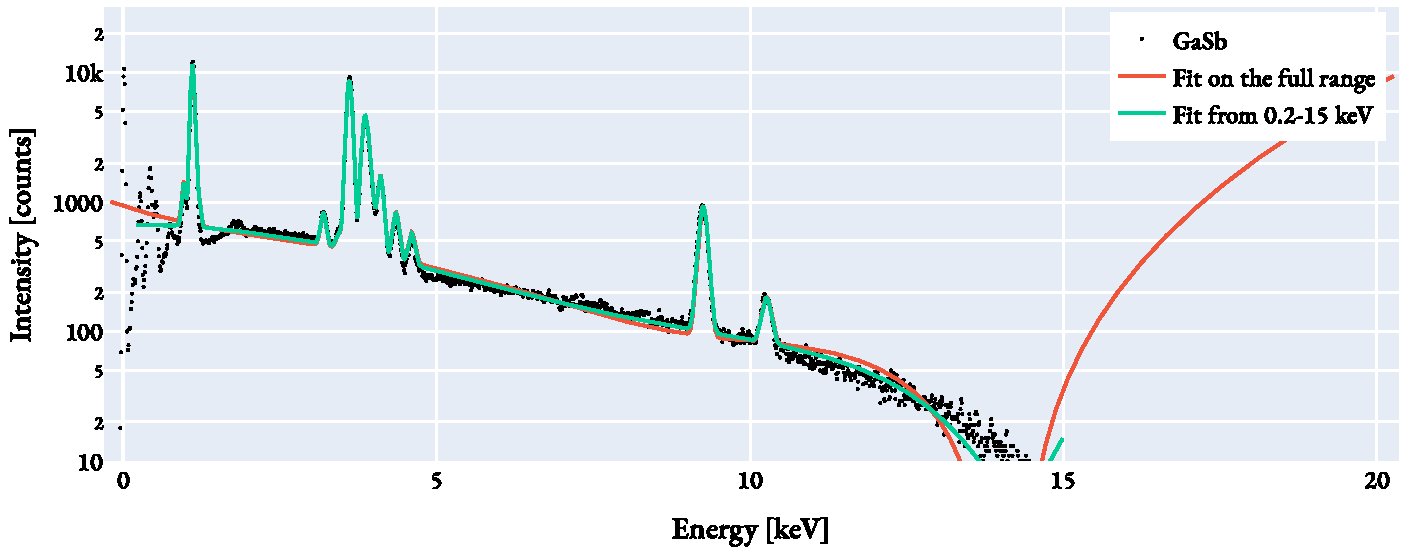
\includegraphics[width=0.85\linewidth]{figures/discussion/model_slicing_fit.pdf}
    \caption{
        Illustration of the effect of slicing the spectra before model fitting.
        Correct slicing of the spectra improve the background fit, and prevents unpredictable results above the beam energy.
        % Slicing out the noise peak and the low energy peaks of no interest will also improve the background fit.
        The sliced fit is the green line, which is not perfect at the very beginning and the end, but good enough around the peaks of interest.
        The red line, fitted on the whole energy range (0-20 keV), fits poorly at the beginning and very poorly at the end.
        The red line is not too bad around the peaks of interest, but fits worse than the green line here.
        The black dots are the data, which are from the 15 kV 50 pA GaSb spectrum.
    }
    \label{fig:discussion:model_slicing_fit}
\end{figure}



% More on artifacts, Si peak, C peak
% the C Ka peak. Contamination?
% no/little O Ka in GaAs.
Some artifacts seem to be affected by the amount of counts, and other artifacts are not.
As mentioned above, the coincidence events are affected by the amount of counts, giving both peaks and tailing counts.
The internal fluorescence Si peak is not affected by the amount of counts as the coincidence events are, and is present at similar low relative intensities in all spectra.
This Si peak is from the detector as explained in \cref{theory:eds:hardware}, and is expected to be present at low levels in all spectra.
The Si signal could also have some contribution from the Si wafer that the specimen is mounted on, the spectra acquired on clean Al specimen stubs in \cite{project_report} also had similar relative amounts of Si.
No other peaks like Fe from the column or the detector are present in the spectra, implying that the collimator on the detector is working as intended by limiting X-rays which originate from other points than the targeted point on the specimen.
The carbon contamination in the form of a C K$\alpha$ peak is present in all spectra.
The absorption is high at low X-ray energies, but the C K$\alpha$ peak is present at similar relative intensities in all spectra.
This C peak can both be from a contamination on the specimen, or from somewhere in the chamber, detector, or column.
The most probable source is contamination on the specimen, as a post acquisition image in panel (b) of \cref{fig:SE_images:GaAs}, taken with the ETD detector, showed darker spots on the acquired areas and a darker square where the specimen was scanned.
The ETD detector combines the SE and BSE signals, and the darker spots are therefore most likely carbon contamination on the specimen.
The image also have some horizontal lines, which are scanning artifacts.
The biggest dark spot, located highest, is from the 30 kV spectrum, showing that the interaction volume is larger at higher beam energies.
The source of the C signal can be further investigated by looking at different specimens, and should be done when low energy lines are of interest.
As the peaks used in this work are from 1 keV and above, the signal from C is not of concern in the remainder of this work.


% O Ka peak
Another artifact observed in the spectra is the O K$\alpha$ peak, which is present in the GaSb spectra, but not in the GaAs spectra.
% However, the O K$\alpha$ peak is only present in the GaSb spectra, and not in the GaAs spectra.
The mass absorption coefficients for GaAs is twice as high at O K$\alpha$ than for GaSb, which could have been the reason for the O K$\alpha$ peak not being present in the GaAs spectra, but then the same should have been true for the C K$\alpha$ peak.
% GaAs: mu_rho(O_Ka) = 7k, mu_rho(C_Ka) = 24k
% GaSb: mu_rho(O_Ka) = 4k, mu_rho(C_Ka) = 11k
Thus, another explanation is needed for the absence of the O K$\alpha$ peak in the GaAs spectra.
It could be due to different contamination on the two specimens, where the GaSb specimen have a thicker oxide layer than the GaAs specimen.
This can both be an effect of the As vs Sb, or the age of the specimens, as the GaSb specimen could have been exposed to air for a longer time than the GaAs specimen.
Another possibility is that the O K$\alpha$ peak is mislabeled, and is actually a Sb M-line.
This option is discussed in the second next paragraph.
\ton{Any other ideas for the 0.5 keV peak?}


% absorption edge effects. suggest future work, splice
Similar absorption edge effects as observed in \cite{project_report} are present in the acquired spectra, where strong absorption edges at lower to medium energy influence the background intensities strongly.
This is illustrated well in \cref{fig:background_absorptionEdgeSi}, where the spectrum is overlaid with the mass absorption coefficient for Si.
The background intensity is reduced by the absorption edge, i.e. the intensity of the background is higher before the peak than after the peak.
This makes the background modelling more difficult, as the background is modelled with a polynomial function.
Lower accuracy in the background modelling could lead to worse quantification, as well as incorrect metrics discussed in this work.
One possible improvement to the background modelling is to use a spline function instead of a single polynomial function.


% Sb M-lines not in any table, but M is stated to be 0.733 keV at https://www.globalsino.com/EM/page4675.html
Another take-away from the qualitative analysis is that the HyperSpy database does not contain the Sb M-lines.
The GaSb spectra have a clear peak at what is assumed to be the Sb M$\eta$ peak around 0.42 keV, based on the qualitative analysis AZtec, as well as the absorption edge in Sb at 0.5 keV.
The energy of a line is located a few eV below the absorption edge.
The online book "Practical electron microscopy" by Y. Liao \cite{liao2006practical} lists a Sb M lines at 0.733 keV, but this is only visible in the spectra as a slight increase in counts and not a real peak.
The HyperSpy database and the X-ray data Booklet \cite{thompson_x-ray_2004} does not list any M-lines below Z=57.
A screenshot from the AZtec software, which identifies two Sb M-lines, one at 0.4 and a smaller at 0.7 keV, is shown in \cref{fig:discussion:AZtec_Mlines}.
The screenshot is of the spectrum with low energy resolution, and the 0.4 and 0.5 keV peak is overlapping, but the AZtec software clearly identifies the leftmost part of the merged peak as a Sb M-line.
This is an indication that the peak at 0.5 keV is not a Sb M-line, but rather that the O K$\alpha$ peak is labeled correctly.
The lack of the Sb M-lines in the HyperSpy database can be a source of error in the quantification, as the Sb M-lines are not included in the background modelling.
A solution to this is to slice off the spectrum before fitting the background so that unavailable lines are excluded from the background modelling.
This requires that the user visually inspect the lower energies thoroughly, and that the user is aware of the possibility of missing lines.
Another solution is to add the Sb M-lines to the HyperSpy database, which would require more research into M-lines of elements with Z lower than 57.

\begin{figure}[htbp]
    \centering
    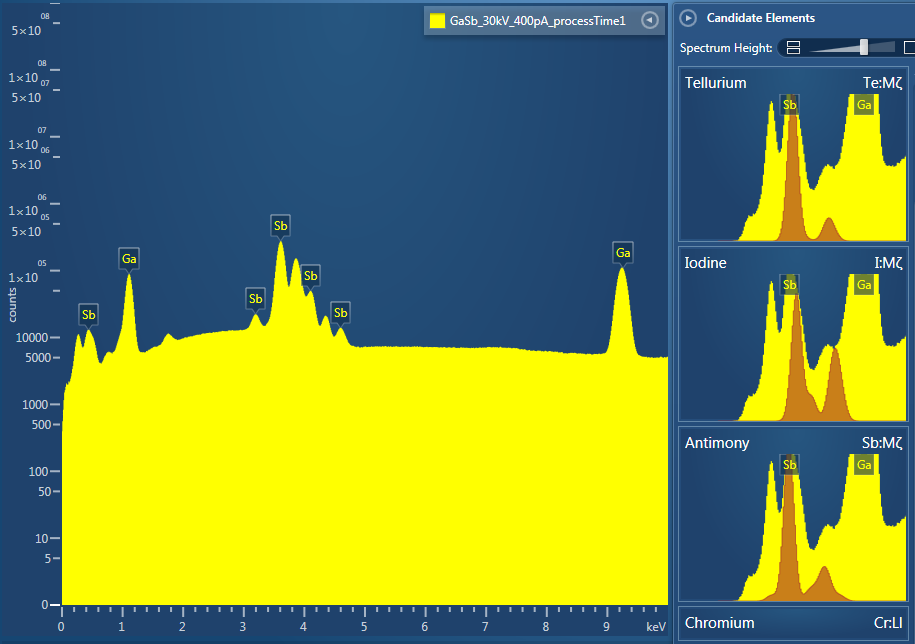
\includegraphics[width=0.95\linewidth]{figures/discussion/AZtec_Mlines.png}
    \caption{
        Screenshot from the AZtec software, showing the Sb M-lines identified at 0.4 and 0.7 keV.
        The right part of the screenshot show that tellurium and iodine match slightly better than antimony, but the L-lines present are definitely from antimony.
        }
    \label{fig:discussion:AZtec_Mlines}
\end{figure}

















\section{Setup metrics}
\label{discussion:setup}

% Same sentence now as results:
The setup metrics measured in this work are energy resolution, the energy scale and offset, peak ratios, and deviations in peak positions.



\subsection{Energy resolution of the detector}
\label{discussion:setup:energy_resolution}


% the first table with energy resolution in a spectrum
\cref{results:setup} begins with a table showing an issue with the calculated energy resolution, which is that in a single spectrum, different reference peaks give different energy resolutions.
The energy resolutions are calculated from the FWHM of different peaks, using \cref{eq:estimateFWHM} by Fiori and Newbury.
Calculated energy resolutions for GaAs and GaSb taken at 30 kV with 50 pA is tabulated in \cref{tab:results:lines_info_30kV_50pA}.
The calculated energy resolutions for GaAs varies from 123 eV to 135 eV, and for GaSb from 121 eV to 133 eV,  when using different peaks as the reference peak.
This illustrates an issue with specifying a single energy resolution for a spectrum.
The energy resolution is supposed to be a property of the detector.
As explained in the theory chapter, the acquisition parameters like ICR and PT affect the achieved energy resolution, but the results here show that the specimen and choices for calculations also affect the energy resolution.
%  data here shows that the energy resolution is also affected by the specimen.
The ISO standard 15632 \cite{iso_qc_15632} on SEM EDS performance parameters is directed towards the manufacturer of the detector, where the described method for measuring the energy resolution is with an $^{55}$Fe source off the microscope.
However, for user laboratories the standard specify that a polished manganese specimen can be used.
This does require that the user laboratory has a polished manganese specimen, which is not the case for the user laboratory in this work.
Possible test specimen is discussed in \cref{discussion:other:test_specimen}.
Measuring directly on a Mn specimen is the first of three possibilities for measuring the energy resolution, introduced in \cref{theory:eds_performance:energyres}.
The second method is to measure the FWHM of Ni K$\alpha$, e.g. with a NiO test specimen from Ted Pella, and then multiply the FWHM by 0.926 to get the FWHM of Mn K$\alpha$.
This method relies on specific specimen, which is expensive and had been ordered but not delivered during the time span of this work.
Other non-standard Ni test specimen could probably be used, but the 0.926 factor is based on NiO test specimen and the results from a round-robin study in 1995 with five TEM laboratories \cite{bennett_egerton_1995}.
The third method, which is given in Goldstein \cite{goldstein_scanning_2018}, is the Fiori and Newbury equation mentioned above.
As neither a Mn specimen nor a NiO specimen was available for this project, the third method was used.
The third method is also more flexible and general, as it does not rely on specific specimen.


% more on energy resolution
Claiming that the energy resolution is a property of the detector, the acquisition parameters, the specimen, and additionally the choices during calculations, raises the question of what the energy resolution actually is.
The energy resolution is a much used comparison metric for EDS detectors, and is thus important.
Having a single number for the energy resolution is convenient, but it is not a complete description of the energy resolution.
Traditionally, the energy resolution is seen as a property of the detector, but the ISO standard 15632 \cite{iso_qc_15632} stress the need for specifying the ICR with the energy resolution, preferably with one number at low ICR and one at high ICR.
When looking at the other acquisition parameters, the data in \cref{tab:results:energy_resolutions} shows a strong dependence on the PT, and a weaker trend with the ICR.
These numbers are calculated with HyperSpy, which use \cref{eq:estimateFWHM}, but selects the reference peak as the alphabetically first $\alpha$ peak.
Both the use of \cref{eq:estimateFWHM} and the choice of reference peak was not documented properly, so the author of this work raised an issue on the HyperSpy GitHub page with a suggestion for improvement with a pull request\footnote{Issue: \url{https://github.com/hyperspy/hyperspy/pull/3099}. Pull request: \url{https://github.com/hyperspy/hyperspy/issues/3098}}.
Regarding the PT, it should be selected to give the best energy resolution, as it is safe to assume that the manufacturer has done this for the specifications of the detector. 
The highest PT gave an energy resolution of 127 eV, while the lowest PT gave 158 eV.
The ICR trend is weaker, indicating that lower ICR gives better energy resolution, but the changes are around $\pm$ 2 eV.
The ICR is dependent on the beam energy and the current, but also on the specimen.
This specimen dependence for the ICR might be one of the factors which make the energy resolution dependent on the specimen.
Another specimen factor is the available lines generated by the elements.
This effect is most apparent when looking at the estimated FWHMs from multiple lines in a single spectrum, as in \cref{tab:results:lines_info_30kV_50pA}.
The shared lines, i.e. Ga L$\alpha$ and Ga K$\beta$, have similar but not identical FWHMs.
Such variations of a few eV are expected with measurement noise, and is very small compared to the peak broadening from the detector, as explained in \cref{theory:eds:hardware}.
The lowest energy resolution for both spectra is from the Ga K$\beta$ line, implying that the Ga K$\beta$ line is narrower than it is "supposed" to be, compared to the other lines.
For GaAs, the explanation could have been that the peak overlap some with As K$\alpha$, but that is not the case for GaSb, and another explanation is needed.
The Ga K$\beta$ peak is much less intense than the other lines used as reference, which can give slightly worse model fit.
Another possibility is that the equation used to estimate the FWHM works better for $\alpha$ lines, but that is contradicted by the As K$\beta$, Sb K$\beta$1, and Sb K$\beta$2 lines.
The most probable cause is the low intensity.
Cherry-picking reference line can give better energy resolution, but it is not a good practice as it is not a general solution.
A solution for the method using \cref{eq:estimateFWHM} could be to average the estimated energy resolution for a fixed set of reference lines.
This would then depend on a standardized test specimen.
Regarding the small variations between spectra with similar or equal acquisition parameters, the cause is probably measurement noise.
Such small variations when measuring the metric are expected, and would probably be solved by averaging over multiple spectra with the same acquisition parameters.
To summarize, the energy resolution of a detector should be specified with the acquisition parameters, the specimen used for the measurement, and the method used for calculating the energy resolution.
Alternatively, a larger uncertainty can be used to specify a more general energy resolution.
An example of the first, based on the results in \cref{tab:results:energy_resolutions}, would be:  the energy resolution of the detector is 127 eV at 30 kV and 50 pA, measured on a GaAs specimen, and calculated with \cref{eq:estimateFWHM} with the Ga K$\beta$ line as reference.
The second way of specifying the energy resolution would be: the energy resolution of the detector is 127 $\pm$ 6 eV at optimal acquisition parameters, measured on a GaAs and GaSb specimen, calculated with \cref{eq:estimateFWHM}.



\subsection{Energy scale and offset, and peak position deviations}
\label{discussion:setup:scale_offset}

The calibration of the spectra was done with HyperSpy, and the results for the energy scale, the offset and the deviations in the peak positions are close to the expected values.
The scale and offset is presented in \cref{tab:results:scale_offset}, and the deviations in \cref{tab:results:lines_info_30kV_50pA} are representative for the peak deviations.
Low deviations for the scale and offset show that the detector is calibrated properly.
The GaAs spectra have one order of magnitude higher standard deviation for the scale than the GaSb spectra, which is probably due more 15 kV and 30 kV spectra for GaSb.
The numbers would probably be more similar if the same number of spectra were used for both specimens.
However, the numbers are still comparable, as the scale and offset is not expected to change with the specimen nor the acquisition parameters.
With a scale of 10 eV, a peak deviation of $\pm$ 2 eV is good, and any better is not necessary as the channel size and energy resolution limits perfect peak position.




\subsection{Peak ratios}
\label{discussion:setup:peak_ratios}

The idea of measuring peak ratios was to get a number for the possible carbon contamination, as it is done in the work of Egerton \cite{egerton_nio_characterization_1994}.
As there is some carbon present in both the GaAs and GaSb spectra, the peak ratios could give a number for the carbon contamination, and the change over time.
However, the metric needs a time series of spectra, where the change in K to L peak ratio is plotted, and an increase in K over time would indicate carbon contamination.
Measuring time series of spectra was not prioritized in this work, as the focus was directed elsewhere.

The peak ratios in \cref{tab:results:peak_ratios} are not an example of a time series, but the ratios are still interesting.
GaSb have around three times higher ratio for Ga K$\alpha$ and Ga L$\alpha$ than GaAs.
The higher ratio either indicates more Ga K$\alpha$ or less Ga L$\alpha$.
The GaAs spectra have much intensity from the As L$\alpha$ peak, which can be absorbed by the Ga L$\alpha$ peak, and thus giving the Ga L$\alpha$ peak a higher relative intensity in the GaAs spectra.
As explained in \cref{theory:xray_formation:characteristic}, the absorption probability is highest right above the absorption edge, and thus the As L$\alpha$ X-rays are absorbed easier than the Sb L$\alpha$ X-rays.
This is an indication of absorption, which will be discussed more in \cref{discussion:bulk_corrections}.











\section{Acquisition parameters}
\label{discussion:acquisition_parameters}

% The performance metrics of the acquisition are: the Duane-Hunt limit, the Fiori peak-to-background ratio, and portion of counts in peaks vs background.
% Additionally, results from the user parameters process time, beam energy, and beam current are presented.

The performance metrics for the acquisition parameters are the Duane-Hunt limit and the Fiori peak-to-background ratio, which is presented with observations for PT, $E_0$, and $i_b$.


\subsection{Process time}
\label{discussion:acquisition_parameters:process_time}

The best PT for a specimen is dependent on the aim of the analysis, as a high PT gives a better spectrum, but takes longer time.
Better spectrum means higher energy resolution and fewer artifacts.
Even though high PT gives a good spectrum, the amount of counts recorded per second is lowered, and thus the DT increase with increasing PT.
The time aspect is especially important when measuring EDS maps, as these can be very time-consuming with a high PT.
As seen in the results, the PT affect the energy resolution, the evenness of the spectrum through the amount of counts, the amount of artifacts with increasing ICR, and the DT. 


% visible seperable vs gaussian modelling
For quantitative analysis, it is probably best to have a high PT, as the energy resolution is better, and the amount of artifacts is lower.
This allows the user and potential automatic detection software to detect and separate peaks easier.
Using automatic detection should be done with caution, as there are cases where peaks are labeled incorrectly.
This is explained and discussed in detail in a paper by D. Newbury \cite{newbury_2005_misidentification}.
Newbury raise concerns about the use of automatic peak detection, with examples of misidentified major constituents.
Such misidentifications are a serious challenge for the credibility to EDS community, and should be avoided when possible.
Acquiring spectra with a high PT limits the possibility of misidentifications, as the peaks are more visible and separable.
% gaussian modelling
When a specimen is labeled correctly, the peaks can be modelled as Gaussian functions.
Model fitting can deal with overlapping peaks quite well, if the right lines are added to the model.
A computer can separate overlapping peaks better than the human eye, and is less dependent on having the best possible energy resolution.


% Specimen dependence
As the process time is very influential on the energy resolution, the best PT for an analysis is dependent on the specimen.
If the specimen have many L lines which are of interest, the PT should be high.
If the peaks of interest are in the higher energy range, the PT can be lower to allow higher throughput.
As seen in panel (c) in \cref{fig:results:energy_resolutions_process_time}, the maximum and minimum PT does not make a big difference for the Ga K$\alpha$ peak, but the Ga L$\alpha$ peak is merged to a visible unseparable peak with Ga L$l$ in panel (a).
However, the Gaussian modelling of the PT 1 spectra separate the low energy peaks, and the quantification is actually the one closest to the expected values.
The quantification results, presented in \cref{fig:results:initial_quantification} and \cref{tab:results:initial_quantification}, show that higher amount of counts can give better quantitative results.


The best general PT is probably high, but not the highest possible.
At 30 kV and 50 pA, PT 6 have DT 44\%, while PT 4 have DT 13\%.
Acquiring a PT 6 spectrum then takes 2-3 times as long as a PT 4 spectrum, and the energy resolution difference is 127 eV vs 132 eV, given in \cref{tab:results:PTvsFWHMs}.
The high increase in DT and acquisition time is in many applications not worth the small improvement of energy resolution.



\subsection{Beam energy and beam current}
\label{discussion:acquisition_parameters:beam_energy_current}

Setting the beam energy and beam current is important for the throughput and the spatial resolution of eventual EDS maps.
The combination of beam energy and beam current is setting the amount of X-rays generated, and thus the amount of counts recorded.
The beam energy is important for the overvoltage, which for example is an issue for the Sb L lines at 5 kV and 10 kV. 
Seen in the voltage series figures (\cref{fig:results:GaAs_voltages,fig:results:GaSb_voltages}), the 15 kV and 30 kV spectra are very similar around 1 keV, but then the 15 kV spectra falls off faster than the 30 kV spectra.
This is probably due to the overvoltage being lower faster at 15 kV than at 30 kV, and thus the ionization cross-section is decreasing faster at 15 kV than at 30 kV.

% the choise of constant current for the voltage series, a bad idea?
The voltage series were acquired with constant beam current, which probably could have been done better with constant input count rate.
The constant beam current was selected to make the spectra as comparable as possible, but the low ICR at 10 kV and 5 kV made the spectra noisy, as an addition to the low overvoltages in these spectra. 
The combination of low beam current and low overvoltage resulted in few counts, and thus not very good spectra.
The idea was to acquire spectra that did not need normalization for good comparison, but a different approach could have solved this better.
Keeping the input rate constant should result in more similar spectra which also does not need normalization, and such an approach can be tested in future works.


% DT as a measurement for artifacts
In the literature (see \cref{theory:eds:user_controlled_parameters}), the DT is given as the parameter that determines the amount of artifacts in the spectrum, but the results in this work do not support this.
The two spectra with the highest DT at 53\% and 77\% had similar amount of artifacts as a spectrum with DT 18\%, and the amount was low.
The mentioned spectra are the GaSb 15 kV and PT 6 spectra, where the DT increase with $i_b$ (50, 200, 400 pA).
These three spectra were very similar, except for the amount of counts, which increase with higher $i_b$.
The spectrum with clearly the most prominent artifacts was the one with the highest amount of counts, recorded at high $i_b$ and low PT, which is the GaSb 30 kV, 400 pA, PT 1 spectrum.
This combination gave around 6-10 times more counts in the peak of interest than the other spectra, but also very clear artifacts.
The spectrum is plotted in \cref{fig:results:overviewGaSb_withArtifacts}, and the artifacts are annotated.
The DT of this spectrum was only 28\%.
The result implies that artifacts are more present when the amount of counts is high and the detector have little time to process the signal.
It might be that the AZtec software is doing some data treatment to reduce the amount of artifacts, and thus that the outputted raw data in the \verb|.emsa| file is not the as "raw" as it is assumed to be.
This is just speculations, as the documentation does not give information about this.
The DT advice given in Goldstein is probably the best one, which states that the analyst should run a test spectrum first to see if the acquisition parameters are suitable for the specimen, without generating too many and intense artifacts.
In other words, the DT is not as useful as a parameter to determine the quality of the spectrum, and should mainly be used when considering the acquisition time.
Other parameters like the count rate and PT should be used to adjust the amount of artifacts, and even though the DT is a product of these parameters, it is not a good measurement for the artifacts.



\subsection{Duane-Hunt limit}
\label{discussion:acquisition_parameters:duane_hunt_limit}


(Low deviations, little to discuss)


\subsection{Fiori peak-to-background ratio}
\label{discussion:acquisition_parameters:fiori_peak_to_background_ratio}

(Much to discuss here. Usefulness, implications for quality, the calculation for the value of comparison.)


(A function of: the detector, the specimen, the line selected, the acquisition parameters, and the calculation method.)












\section{Bulk corrections}
\label{discussion:bulk_corrections}



\dots










\section{Other discussions}
\label{discussion:other}

\subsection{Test specimen}
\label{discussion:other:test_specimen}

\subsection{SEM EDS standards}
\label{discussion:other:sem_eds_standards}

\subsection{Flatness of the specimen surface}
\label{discussion:other:flatness}

\subsection{Other metrics}
\label{discussion:other:other_metrics}




















%%%%%%%%%%%%%%%%%%%%%%%%%%%%%%%%%%%%%%%%%%%%%%%%%%%%%%%%%%%%%%%%%%%%%%%%%%%%%%%%%%%%%%%%%%%%%%%%%%%%%%%%%%%%%%%%%%%%%%%%%%%%%%%%%%%%%%%%%%%%%%%%%%%%%%%%%%%%%%%%%%%%%%%%%%%%%%%%%%%%%%%%%%%%%%%%%%%%%%%%%%%%%%%%%%%%%%%%%%%%%%%%%%%%%%%%%%%%%%%%%%%%%%%%%%%%%%%%%%%%%%%%%%%%

% This was in the old file:

%%%%%%%%%%%%%%%%%%%%%%%%%%%%%%%%%%%%%%%%%%%%%%%%%%%%%%%%%%%%%%%%%%%%%%%%%%%%%%%%%%%%%%%%%%%%%%%%%%%%%%%%%%%%%%%%%%%%%%%%%%%%%%%%%%%%%%%%%%%%%%%%%%%%%%%%%%%%%%%%%%%%%%%%%%%%%%%%%%%%%%%%%%%%%%%%%%%%%%%%%%%%%%%%%%%%%%%%%%%%%%%%%%%%%%%%%%%%%%%%%%%%%%%%%%%%%%%%%%%%%%%%%%%%

% Flatness of the specimen surface
% check out: Newbury and Ritchie 2013, Quantitative SEM/EDS, Step 1: What Constitutes a Sufficiently Flat Specimen?
% https://www.cambridge.org/core/services/aop-cambridge-core/content/view/E9E18A67EED08A3A7F23C4559F81DE93/S1431927613008210a.pdf/quantitative-semeds-step-1-what-constitutes-a-sufficiently-flat-specimen.pdf





% \section{Regarding the ISO 15632 standard}
% \label{theory:eds_performance:iso15632}

% BAM (Federal Institute for Materials Research and Testing) has a test sample for SEM EDS with a accompanying software, which satisfies the ISO 15632 standard.
% However, the price per 28.02.2023 for this sample (EDS TM002) is 334 EUR and 335 EUR for the software.
% A full test in accordance with the ISO standard could probably be done with a cheaper sample and a Jupyter Notebook, where the user would see all the steps and the results.
% This has not been a main focus in this work, but some parameters in the ISO standard are covered in this work.

% \url{https://webshop.bam.de/webshop_de/eds-tm002.html}

% paper at \url{https://www.cambridge.org/core/services/aop-cambridge-core/content/view/17A1D769BB6B9B76B5AC815911FAE7FD/S1431927613008271a.pdf/check-and-specification-of-the-performance-of-eds-systems-attached-to-the-sem-by-means-of-a-new-test-material-eds-tm002-and-an-updated-evaluation-software-package-eds-spectrometer-test-version-3-4.pdf}





% TODO: energy resolution. the older xmax info claims high energy resolution and high cps. The x-max-N datasheet lists resolution with cps, which is nicer. Progress.




% \section{Qualitative analysis}
% \label{method:qualitative_analysis}

% See Annex A in ISO 22309. Also make a notebook, which can be shared with HyperSpy people.
% Show the use of find_peak_ohaver, referring to O'Haver's paper, with different settings.
% Also show nice plotly plots, eventually plt with plotting all lines in HS for the element.
% And maybe also fitting, where the area is shown to see if any added elements are 0.
% Can refer to autoID, and it's flaws.

% Rule for what a peak is? See eg Annex A in ISO 22309: I > (BG + 3 x sqrt(BG)), wher BG is mean of BG (probably at the given energy)

% \brynjar{ISO 22309: "typically a value of 30 eV can be critical; peaks separated by more than this figure should not be confused by either automatic or manual identification procedures."}





% \subsection{Calibration}
% \label{method:calibration}

% For some reason, it works better to calibrate the offset and then the scale/dispersion.
% HyperSpy allows for calibration of offset, scale or energy resolution, but only one at a time.
% The procedure used was: calibrate offset, calibrate scale, recaliabrate offset, and recalibrate scale.
% After the recalibration, the difference was compared to the first calibration, and if the change was more than 5\%, the calibration was repeated.
% By default, the HyperSpy calibration uses all alpha lines.
% It is possible to specify certain lines to calibrate on, but this yeilded the same or worse results as using all alpha lines.
% \brynjar{The stuff above is more discussion, at least the last sentence.}






% \subsection{The requirements for a standard material}
% \label{theory:eds_performance:standard_material}
% smt about the standard materials available \dots
% what we want in the spectrum \dots
% candidates \dots







% \subsection{Other tests - not used in this work}
% \label{theory:eds_performance:other}

% \brynjar{TODO from Ton: "if not used, do not include them. But consider to use them in discussion leading to concrete future work (last chapter)"}

% Other test are described in the literature, but they were not used in this work.
% Some of them is mentioned here, either because they are interesting but not possible, because they are not relevant enough, or because they could be relevant in future works.

% \subsubsection*{Linearity and stability}
% In Goldstein \cite[p. 232]{goldstein_scanning_2018} it is stated that the two most important tests for an EDS detector are linearity and stability.
% This is stated in the section about what to look for when buying a detector.
% The reason for not including these two test in the work is mainly their dependence on a way to measure the probe current, which e.g. can be done with a Faraday cup.
% Such tests could be used in the future and are therefore briefly described here.
% Linearity of the detector is that the number of X-rays measured is proportional to the number of X-rays generated.
% Stability is that the detector resolution and the peak positions does not change significantly with different probe currents.
% Both tests require multiple spectra of the same sample with different probe currents.
% The ISO 22309 standard on quantification of EDS spectra \cite{iso_quantification_22309} also mentions these two tests.

% % \brynjar{ISO 22309: "Whatever type of detector is being used, the count rate capabilities of the system should be checked by
% %     comparing a spectrum obtained at a count rate below 2 000 counts/s with a spectrum obtained at the highest
% %     count rate to be used, to look for peak shift and pile-up distortion that might affect relative peak heights. A
% %     minimum of two checks on beam stability, using a Faraday cup, or a known reference specimen, should be
% %     made prior to and following the analysis."}

% % TODO : kan jeg gjøre de med beam current???



% \subsubsection*{Peak shape}

% Deviations of peak shapes can be used to identify problems with the detector or the qualitative analysis.
% Peak shapes are used in Egerton and Chengs work to identify incomplete charge collection, but this is a lesser concern in modern SDDs.
% Peak shapes deviating from a Gaussian shape, which is not due to detector issues, are probably due to misidentification where a minor peak is not correctly identified.
% The overlapping peak has the counts from both peaks, and the shape will be skewed.
% Assessing the peak shape with numbers is not straightforward, but the FWHM/FWTM can be used to compare the peak shape of different spectra.
% This requires the peaks to be standing alone, without any overlap.
% As this is not always the case, and that the metric is not too useful, it is not used in this work.
% However, an analyst should be aware of the peak shape, as it can be useful if a skewed peak is found and lacking a clear explanation.

% Overlapping peaks, ASTM 1508:
% "9.2.5 Next look for peak overlaps. If (1) a peak is displaced
% relative to its marker, (2) relative intensities are wrong, or (3)
% there is a distortion in the peak shape, then there is an
% overlapping element. All three conditions will be present in an
% overlap situation."


% \subsubsection*{Shadowing}
% \brynjar{From ISO 15632: "In many cases the specific geometry of the EDS detector at a particular SEM/EPMA chamber can result in a reduction of the net active sensor area as expected after subtraction of shadowing area caused by the window grid. For example, a falsely mounted collimator, electron trap or shadowing by other parts in the SEM chamber can reduce additionally the illumination of the detector with X-rays. A practical procedure how to determine experimentally the effective area of an EDS detector and under which conditions are described in Reference [5]."}
% % [5] Procop M., Hodoroaba V.-D., Terborg R., Berger D., Determination of the Effective
% % Detector Area of an Energy-Dispersive X-Ray Spectrometer at the Scanning Electron
% % Microscope Using Experimental and Theoretical X-Ray Emission Yields, Microsc. Microanal.,
% % 22 (2016), pp. 1360-1368
% % Shadowing



% \subsubsection*{Energy dependence of instrumental detection efficiency - K/L ratio}
% \brynjar{ISO 15632: "The minimum specification for the energy dependence of the instrumental detection efficiency shall be
%     the intensity ratio of a low energy line and a high energy line in the characteristic X-ray spectrum of a
%     given material. This ratio shall be given as the net peak area of the L series lines divided by the net peak
%     area of K$\alpha$ series lines in the spectrum of a pure nickel or copper specimen, excited by a 20 keV electron
%     beam perpendicular to the specimen surface and collected by the detector at a take-off angle of 35 degrees. The
%     specimens to be used, the measurement conditions, the calculation of L/K ratio and its conversion for
%     TOA not equal 35 degrees are given in Annex B. \dots These measures are only appropriate for a detector thick enough to absorb at least 95 % of the incident
%     X-ray energy at 8 keV."}


% \subsubsection*{Optimal WD}
% \url{https://www.cstl.nist.gov/div837/837.02/epq/dtsa2/FaultsFoiblesEDS.pdf}
% % \brynjar{En geometri-greie. Er det forskjellig for ulike materialer? Passer under acquisition params}